\subsection{Deep Neural Networks for Acoustic Modeling in Speech Recognition \cite{Hinton2012Deep}}

This paper provides an overview of the progress of acoustic modeling by \emph{deep neural networks (DNNs)}. It also presents the shared view of four research groups (groups at the University of Toronto, Microsoft Research, Google, and IBM Research) that have had recent successes in using this technique.

The goal of the acoustic modeling in this paper is to determine how well each state of a \emph{hidden Markov model (HMM)} fits a frame or a short window of frames of coefficients that represents the acoustic input $p(HMMstate | AcousticInput)$. So the produced acoustic model is combined with the classic HMM to form the final hybrid \emph{automatic speech recognition (ASR)} system.

In modern ASR systems, the acoustic input is typically represented by concatenating \emph{Mel-frequency cepstral coefficients (MFCCs)} or \emph{perceptual linear predictive coefficients (PLPs)}, computed from the raw waveform and their first- and second-order temporal differences. The preprocessing techniques are designed to discard the large amount of information in waveforms that is considered to be irrelevant for discrimination.

The DNN approach for acoustic modeling has two key stages. In the first stage, layers of feature detectors are initialized, one layer at a time, by fitting a stack of generative models. In the second stage, each generative model in the stack is used to initialize one layer of hidden units in a DNN. Finally the whole network is then discriminatively fine-tuned to predict the target HMM states.

The idea behind the first stage is generative pretraining: it finds a region of the weight-space that allows the discriminative fine-tuning to make rapid progress, and it also significantly reduces overfitting. The generative model in DNN approaches uses a set of parameters, $W$, to define the joint probability of a vector of observable variables $v$, and a vector of latent variables $h$, via an energy function $E$:
$$p(v,h; W) = \frac{1}{Z} e^{-E(v,h; W)}, Z = \sum_{v', h'} e^{-E(v', h'; W)}.$$
In the classic \emph{restricted Boltzmann machine (RBM)} which consists of a layer of stochastic binary visible units and a layer of stochastic binary hidden units, the energy function is defined to be:
$$E(v,h) = -\sum_{i \in  visible} a_i v_u - \sum_{j \in hidden} b_j h_j - \sum_{i,j} v_i h_i w_{ij},$$
where $v_i, h_j$ are the binary states of visible unit $i$ and hidden unit $j$, $a_i, b_j$ are their biases, and $w_{ij}$ is the weight between them. The training of a RBM can be achieved by the \emph{contrastive divergence (CD)} algorithm.

After training an RBM on the data, the inferred states of the hidden units can be used as data for training another RBM that learns to model the dependencies between the hidden units of the first RBM. This can be repeated many times to produce many layers of nonlinear feature detectors, which is called a \emph{deep believe network (DBN)}.

\begin{figure}[htbp]
  \centering
  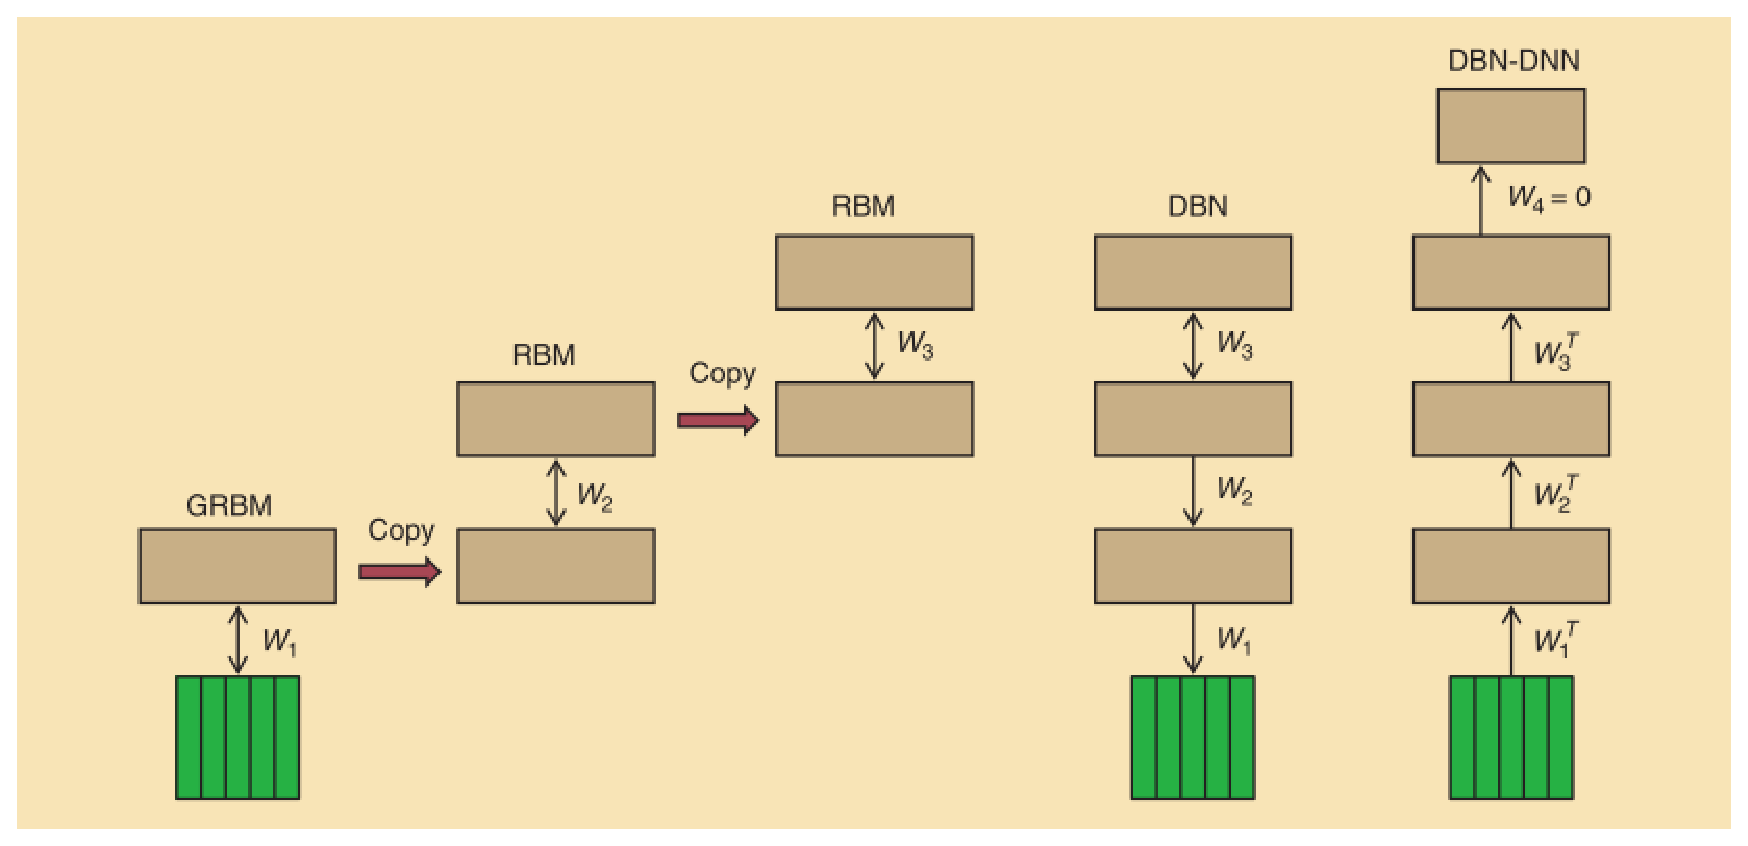
\includegraphics[width=.9\linewidth]{10_17_HMM_DNN}\\
  \caption{Illustration of the DNN training process}\label{fig:HMM_DNN}
\end{figure}

After learning a DBN by training a stack of RBMs, the generative weights in the reverse direction are used as the initialization of a feedforward DNN. It then adds a final softmax layer and trains the whole DNN discriminatively. The whole architecture is illustrated in Figure \ref{fig:HMM_DNN}: 1) A \emph{Gaussian RBM (GRBM)} is trained to model real-valued acoustic coefficients. Then the hidden states of the GRBM are used as data for training the next RBM. 2) This is repeated to create as many hidden layers as desired. 3) Finally, a pretrained DBN-DNN is created by adding a softmax output layer that predicts the hidden state of the HMM.

In the experimental study, the paper reports the results on the TIMIT benchmark and on several large-vocabulary speech recognition datasets. For example in the Bing-voice-search speech recognition task, the best DNN-HMM acoustic model achieves a sentence accuracy of 69.6\% on the test set, compared with 63.8\% for a strong HMM baseline method. 